% !TEX options=--shell-escape
	\documentclass{article}
	\usepackage{amsmath,amssymb}
	\usepackage[inline]{enumitem}
	\usepackage{blindtext}
	\usepackage{booktabs}
	\usepackage{graphicx}
	\usepackage{xcolor}
	\usepackage[vmargin = 1.5in, top = 1in, bottom = 1.2in, letterpaper]{geometry}
	\usepackage{listings}
	\usepackage{courier}
	\usepackage{multicol}
	\usepackage{multirow}
	\usepackage{bm}
	\usepackage[labelformat=simple]{subcaption}
	\renewcommand\thesubfigure{(\alph{subfigure})}
	\usepackage{minted}
	\usepackage{fvextra}
	\definecolor{bg}{rgb}{0.95,0.95,0.95}
	\newminted{r}{mathescape, breaklines, linenos = true, bgcolor = bg, fontsize = \footnotesize}
	\usemintedstyle{tango}
	% \lstset{
	% basicstyle = \small\tt,
	% keywordstyle = \tt\color{blue},
	% commentstyle = \it\color[cmyk]{1,0,1,0},
	% stringstyle = \tt\color[RGB]{128,0,0},
	% %frame = single,
	% backgroundcolor = \color[RGB]{245,245,244},
	% breaklines,
	% extendedchars = false,
	% xleftmargin = 2em,
	% xrightmargin = 2em,
	% aboveskip = 1em,
	% tabsize = 4,
	% showspaces = false
	% }
	\newcommand\inner[2]{\left\langle{#1},{#2}\right\rangle}
	\DeclareMathOperator{\Corr}{Corr}
	\DeclareMathOperator{\Cov}{Cov}
	\DeclareMathOperator{\Var}{Var}
	\DeclareMathOperator{\E}{E}



	\begin{document}
	
	% \newfontfamily\courier{Courier New}

	
	\title{STAT 501 Homework 7
	}
	\author{Multinomial}
	\maketitle
	
	\begin{enumerate}[leftmargin = 0 em, label = \arabic*., font = \bfseries]
	\item
	We use \verb|testnormality| and \verb|mvnorm.etest| to test multivariate normality for each of the 5 groups.
\begin{rcode*}{fontsize = \footnotesize}
load("GRB-5groups.rda")
GRB$class <- as.factor(GRB$class)
source("testnormality.R")
library(energy)
library(dplyr)

# 1.
GRB %>% group_by(class) %>% do(data.frame(testnormality = testnormality(.[,-1]), 
                                          energytest = mvnorm.etest(.[,-1], R = 999)$p.value))
\end{rcode*}
	The result is shown in a table, each row is a group and the \verb|testnormality| and \verb|energytest| are p-values of the tests.
\begin{rcode}
  class testnormality energytest
  <fct>         <dbl>      <dbl>
1 1          1.37e-11         0.
2 2          1.56e- 7         0.
3 3          1.83e-11         0.
4 4          3.55e- 7         0.
5 5          4.21e- 6         0.
\end{rcode}
We can see from the table, the p-values of these two tests are small for all 5 groups, so we conclude that none of the 5 groups are from multivariate normal distribution.

\item 
With equal prior probabilities and costs of misclassification, the Fisher's linear discriminant function is: we allocate $\bm x_0$ to class $k$ if 
\[(\bm \mu_k - \bm \mu_j)^T \bm \Sigma^{-1} \bm x_0 - \frac{1}{2} (\bm \mu_k - \bm \mu_j)^T \bm \Sigma^{-1} (\bm \mu_1 + \bm \mu_2) > 0,\, \forall j \neq k\]
\begin{enumerate}
	\item 
	We use \verb|lda| to find linear discriminant coordinates and displayed the first two in Figure~\ref{lda}, where the numbers indicates the true classes and colors indicates the predicted classes. From the proportion of trace, we can see the first two LDs are important.
	\begin{rcode}
# 2.
library(MASS)
GRB.lda <- lda(class ~ ., data = GRB, prior = rep(1/5, 5), CV = F)

plot(predict(GRB.lda)$x[,c(1,2)], pch = as.character(GRB$class), col = as.character(predict(GRB.lda)$class))
	\end{rcode}
	Result of \verb|lda|:
	\begin{rcode}
Call:
lda(class ~ ., data = GRB, prior = rep(1/5, 5), CV = F)

Prior probabilities of groups:
  1   2   3   4   5 
0.2 0.2 0.2 0.2 0.2 

Group means:
         T50         T90        F1        F2        F3        F4       P64         P256       P1024
1  0.7161427  1.09999449 -6.866703 -6.755047 -6.303286 -5.970475 0.1076258 -0.003654604 -0.15569922
2  0.8767503  1.43435781 -5.911697 -5.764700 -5.272722 -5.167775 0.8160456  0.781044750  0.68898510
3  1.2404441  1.66702134 -6.271358 -6.178697 -5.776086 -5.860244 0.1346726  0.068283039  0.01101267
4 -0.6248785 -0.06790308 -7.979436 -7.770887 -7.052427 -6.489657 0.4285974  0.127604005 -0.35581193
5 -0.7434956 -0.37041146 -7.901950 -7.607295 -6.820649 -6.444810 0.4985062  0.316373558 -0.12758329

Coefficients of linear discriminants:
              LD1        LD2         LD3        LD4
T50   -0.11140679  0.5251030   1.9297123 -0.9854645
T90   -0.03827327  0.3970489  -3.2310124  0.7749042
F1    -0.46531093  0.5711469  -0.1632299  0.3176527
F2    -1.19900658 -0.5821010   0.2746655 -1.2768597
F3     0.26976994 -0.7932447   1.0083814  4.2040301
F4     0.17174454  0.1467376  -0.1972441 -1.5753747
P64    1.44760871  6.0739405 -10.6699427  0.0576076
P256   6.18726628 -9.2732590  10.3833981  3.0383037
P1024 -6.89112833  1.5003026  -2.0483281 -5.0926131

Proportion of trace:
   LD1    LD2    LD3    LD4 
0.8292 0.1084 0.0537 0.0087 
	\end{rcode}

	\begin{figure}[!htb]
		\centering
		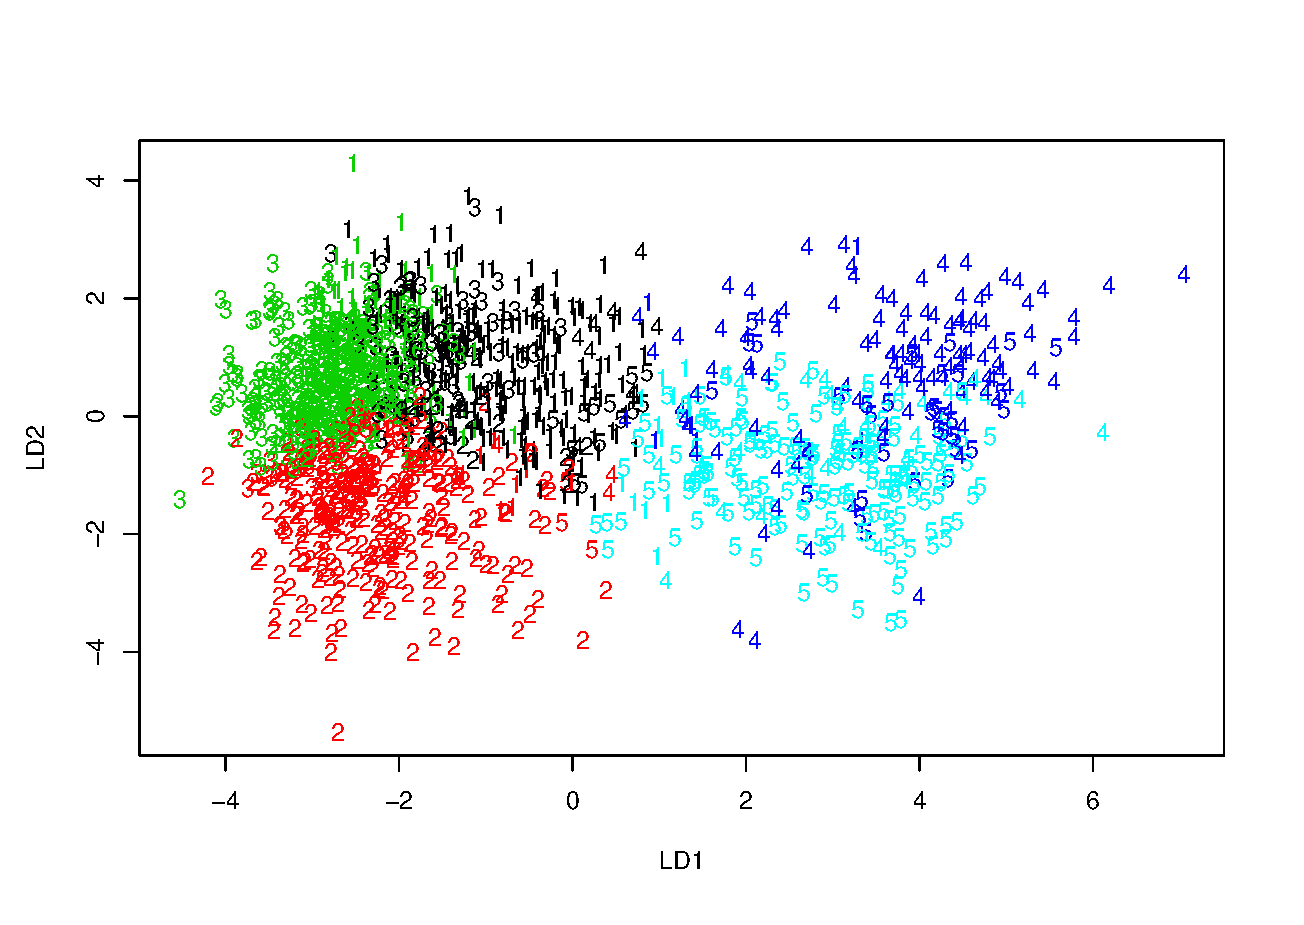
\includegraphics[width = 0.7\textwidth]{Lda.eps}
		\caption{Display of first two linear discriminant coordinates}
		\label{lda}
	\end{figure}

	\item 
	We calculate missclassification rates from AER and LOOCV.
	\begin{rcode}
# AER
mean(GRB$class!=predict(GRB.lda)$class) 
# [1] 0.2307692

# CV
GRBcv.lda <- lda(class ~ ., data = GRB, prior = rep(1/5, 5), CV = T)
mean(GRB$class!= GRBcv.lda$class) 
# [1] 0.235147
	\end{rcode}
	And we got 
	\begin{align*}
	&\mathrm{AER} = \textbf{0.2307692}\\
	&\mathrm{LOOCV} = \textbf{0.235147}
	\end{align*}
	
\end{enumerate}

\item
For QDA:

\begin{rcode}
# QDA
GRB.qda <- qda(class ~ ., data = GRB, prior = rep(1/5, 5), CV = F)
# AER
mean(GRB$class!=predict(GRB.qda)$class) 
# [1] 0.02814259

# CV
GRBcv.qda <- qda(class ~ ., data = GRB, prior = rep(1/5, 5), CV = T)
mean(GRB$class!=GRBcv.qda$class) 
# [1] 0.03689806
\end{rcode}

For k-NN:

We first find the optimal $k$ among $\{1,2,\ldots, 10\}$ with leave-one-out cross-validation (function \verb|knn.cv| is used). The cross valication error rate for each $k$ is shown in Figure~\ref{knn}. From Figure~\ref{knn} we can see $k = 5$ is the optimal one, and we use $k = 5$ to calculate our AER here.
\begin{rcode}
# k-NN
library(class)
# using cross-validation to pick k
# scale the GRB first
GRB.scaled <- scale(GRB[,-1])
# try k = 1,..,10
knn.cv.err<-NULL
knn.cv.sd<-NULL
for (i in 1:10) { 
  temp<-NULL
  for (j in 1:10000)
    temp <- c(temp,mean(knn.cv(GRB.scaled,
                               cl = GRB$class, k = i) != GRB$class))
  knn.cv.err<-c(knn.cv.err,mean(temp))
  knn.cv.sd<-c(knn.cv.sd,sd(temp))
  cat("\n Done i= ",i)
}


plot(knn.cv.err, xlim = c(1, 10),
     ylim=c(min(knn.cv.err - 1.96 * knn.cv.sd),
            max(knn.cv.err + 1.96 * knn.cv.sd)), type = "n")
lines(knn.cv.err + 1.96 * knn.cv.sd, lty = 2, col = "blue")
lines(knn.cv.err - 1.96 * knn.cv.sd, lty = 2, col = "green")
lines(knn.cv.err, col = "red")

# use k = 5
GRB.knn <- knn(train = GRB.scaled, test = GRB.scaled, cl = GRB$class, k = 5)

#AER
mean(GRB.knn != GRB$class)
# [1] 0.1544715

#CV
knn.cv.err[5]
# [1] 0.2142101
\end{rcode}
\begin{figure}[!htb]
	\centering
	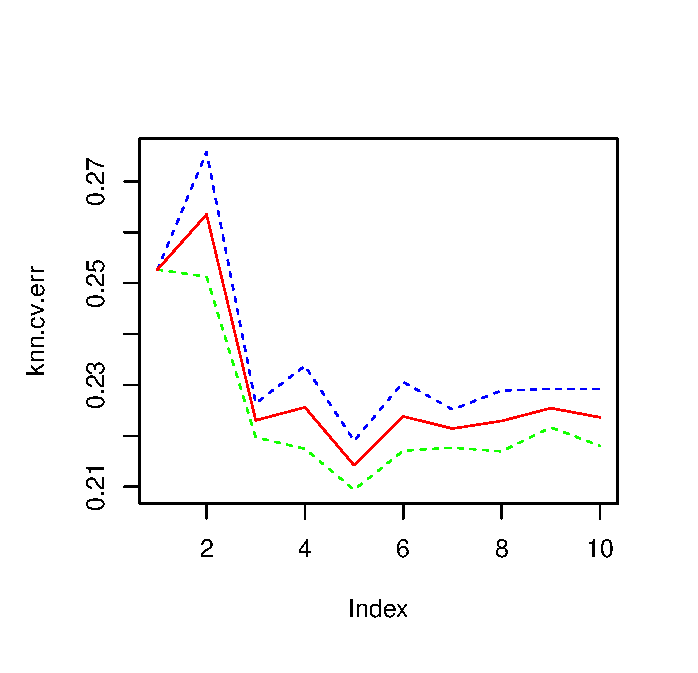
\includegraphics[width = 0.6\textwidth]{Kin.eps}
	\caption{leave-one-out cross-validation error rate for different $k$ and 95\% confidence band}
	\label{knn}
\end{figure}

For CART:

We first find the optimal tree among $\{1,2,\ldots, 10\}$ with leave-one-out cross-validation (function \verb|cv.tree| is used). From Figure~\ref{tree} we can see when number of nodes is 10, we got the optimal tree (which is exactly the one we obtained fron \verb|tree|). Then we calculated AER with this tree. 
\begin{rcode}
#CART
library(tree)
# getting optimal tree using cross-validation
GRB.tree <- tree(formula = class ~ ., data = GRB)
GRB.tree.cv <- cv.tree(GRB.tree, K = nrow(GRB))

# the best one is 10. Plot the best one.
plot(GRB.tree)
text(GRB.tree)

#AER 
mean(apply(predict(GRB.tree), 1, which.max)!=GRB$class)
# [1] 0.286429

#CV
mean(sapply(1:nrow(GRB), function(x) mean(mean(apply(predict(tree(class ~ ., data = GRB[-x,]), newdata = GRB[,-1]), 1, which.max)!=GRB$class))))
#[1] 0.2863993
\end{rcode}
\begin{figure}[!htb]
	\centering
	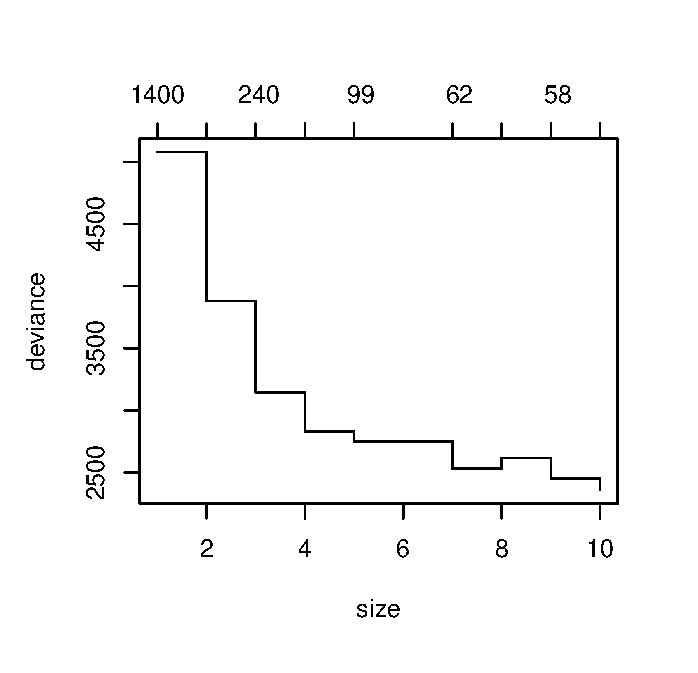
\includegraphics[width = 0.6\textwidth]{Tree.eps}
	\caption{Finding the optimal tree}
	\label{tree}
\end{figure}

\begin{figure}[!htb]
	\centering
	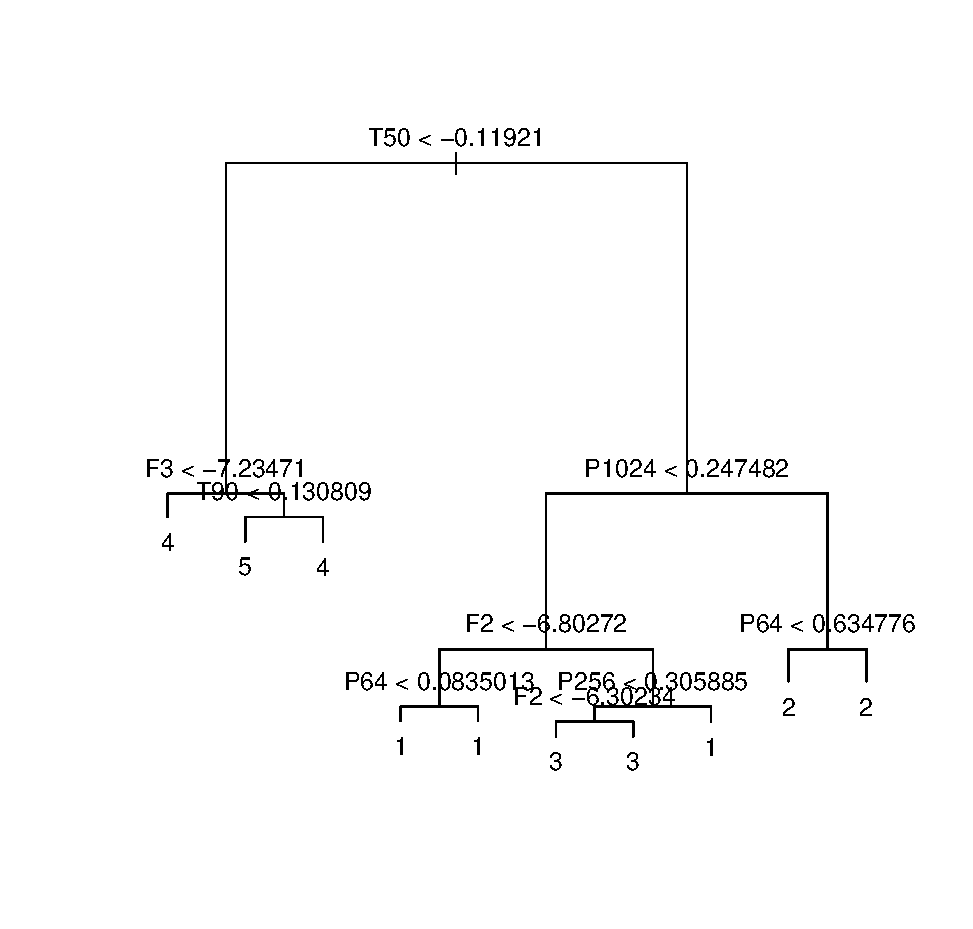
\includegraphics[width = 0.6\textwidth]{Treeopt.eps}
	\caption{Optimal tree}
	\label{tree_opt}
\end{figure}

Now we summarise the missclassification rates with AER and LOOCV in the Table~\ref{miscr} below. From the table, we can see that QDA gives the smallest AER and LOOCV. Thus for this data set, we can use QDA as a classification rule as it out-performs others.

\begin{table}
\caption{Summary of missclassification rates}
\label{miscr}
\begin{center}
\begin{tabular}{ccccc}
\toprule
  & LDA & QDA & k-NN & CART \\
  \midrule
AER & 0.2307692 & 0.02814259 & 0.1544715 & 0.286429\\
LOOVA & 0.235147 & 0.03689806 & 0.2142101 & 0.2863993\\
\bottomrule
\end{tabular}\end{center}
\end{table}


\item 
With 9 variable here, we can only test that $k$ factors are sufficient when $k = 1,2,3,4,5$ (otherwise R will raise an error). Then for each group, we conducted tests when number of factors are 1 to 5. (In some test the p-value cannot be calculated because of errors from function \verb|factanal|. So we put \verb|NA| there for those p-values).
\begin{rcode}
pval_sufficient_factors <- function(data, n){
  tryCatch(factanal(data[,-1], factors = n, rotation = "varimax")$PVAL, error = function(e) NA)
}
GRB %>% group_by(class) %>% do(data.frame(pval_1f = pval_sufficient_factors(., n = 1),
                                          pval_2f = pval_sufficient_factors(., n = 2),
                                          pval_3f = pval_sufficient_factors(., n = 3),
                                          pval_4f = pval_sufficient_factors(., n = 4),
                                          pval_5f = pval_sufficient_factors(., n = 5)))
\end{rcode}
The result is:
\begin{rcode}
# A tibble: 5 x 6
# Groups:   class [5]
  class   pval_1f   pval_2f    pval_3f    pval_4f  pval_5f
  <fct>     <dbl>     <dbl>      <dbl>      <dbl>    <dbl>
1 1     0.        6.33e-102  2.81e- 46  4.21e-  6 5.06e- 3
2 2     0.        1.89e-268  6.27e-154  5.11e-103 3.85e-87
3 3     0.        8.36e-264 NA         NA         3.56e- 8
4 4     3.33e-126 1.78e- 29  6.16e- 14  1.12e-  1 2.72e- 1
5 5     0.        3.42e-125  1.68e- 34  5.71e- 25 4.43e-20
\end{rcode}

We can see from the result that most of the p-values are small. Only the p-values for the test of number of factors being 4 and 5 for class 4 are larger than 0.05. So we conclude that for class 4, 4 factors might be adequate, while for other classes a fewer number of factors is not going to be adequate. 

 \end{enumerate}









	
	
	
	\end{document}